% !Mode:: "TeX:UTF-8"
\documentclass[12pt,a4paper]{article}

%%%%%%%%------------------------------------------------------------------------
%%%% 日常所用宏包

%% 控制页边距
% 如果是beamer文档类, 则不用geometry
\makeatletter
\@ifclassloaded{beamer}{}{\usepackage[top=2.5cm, bottom=2.5cm, left=2.5cm, right=2.5cm]{geometry}}
\makeatother

%% 控制项目列表
\usepackage{enumerate}

%% 多栏显示
\usepackage{multicol}

%% 算法环境
\usepackage{algorithm}  
\usepackage{algorithmic} 
\usepackage{float} 

%% 网址引用
\usepackage{url}

%% 控制矩阵行距
\renewcommand\arraystretch{1.4}

%% hyperref宏包,生成可定位点击的超链接,并且会生成pdf书签
\makeatletter
\@ifclassloaded{beamer}{
\usepackage{hyperref}
\usepackage{ragged2e} % 对齐
}{
\usepackage[%
    pdfstartview=FitH,%
    CJKbookmarks=true,%
    bookmarks=true,%
    bookmarksnumbered=true,%
    bookmarksopen=true,%
    colorlinks=true,%
    citecolor=blue,%
    linkcolor=blue,%
    anchorcolor=green,%
    urlcolor=blue%
]{hyperref}
}
\makeatother



\makeatletter % 如果是 beamer 不需要下面两个包
\@ifclassloaded{beamer}{
\mode<presentation>
{
} 
}{
%% 控制标题
\usepackage{titlesec}
%% 控制目录
\usepackage{titletoc}
}
\makeatother

%% 控制表格样式
\usepackage{booktabs}

%% 控制字体大小
\usepackage{type1cm}

%% 首行缩进,用\noindent取消某段缩进
\usepackage{indentfirst}

%% 支持彩色文本、底色、文本框等
\usepackage{color,xcolor}

%% AMS LaTeX宏包: http://zzg34b.w3.c361.com/package/maths.htm#amssymb
\usepackage{amsmath,amssymb}
%% 多个图形并排
\usepackage{subfig}
%%%% 基本插图方法
%% 图形宏包
\usepackage{graphicx}
\newcommand{\red}[1]{\textcolor{red}{#1}}
\newcommand{\blue}[1]{\structure{#1}}
\newcommand{\brown}[1]{\textcolor{brown}{#1}}
\newcommand{\green}[1]{\textcolor{green}{#1}}


%%%% 基本插图方法结束

%%%% pgf/tikz绘图宏包设置
\usepackage{pgf,tikz}
\usetikzlibrary{shapes,automata,snakes,backgrounds,arrows}
\usetikzlibrary{mindmap}
%% 可以直接在latex文档中使用graphviz/dot语言,
%% 也可以用dot2tex工具将dot文件转换成tex文件再include进来
%% \usepackage[shell,pgf,outputdir={docgraphs/}]{dot2texi}
%%%% pgf/tikz设置结束


\makeatletter % 如果是 beamer 不需要下面两个包
\@ifclassloaded{beamer}{

}{
%%%% fancyhdr设置页眉页脚
%% 页眉页脚宏包
\usepackage{fancyhdr}
%% 页眉页脚风格
\pagestyle{plain}
}

%% 有时会出现\headheight too small的warning
\setlength{\headheight}{15pt}

%% 清空当前页眉页脚的默认设置
%\fancyhf{}
%%%% fancyhdr设置结束


\makeatletter % 对 beamer 要重新设置
\@ifclassloaded{beamer}{

}{
%%%% 设置listings宏包用来粘贴源代码
%% 方便粘贴源代码,部分代码高亮功能
\usepackage{listings}

%% 设置listings宏包的一些全局样式
%% 参考http://hi.baidu.com/shawpinlee/blog/item/9ec431cbae28e41cbe09e6e4.html
\lstset{
showstringspaces=false,              %% 设定是否显示代码之间的空格符号
numbers=left,                        %% 在左边显示行号
numberstyle=\tiny,                   %% 设定行号字体的大小
basicstyle=\footnotesize,                    %% 设定字体大小\tiny, \small, \Large等等
keywordstyle=\color{blue!70}, commentstyle=\color{red!50!green!50!blue!50},
                                     %% 关键字高亮
frame=shadowbox,                     %% 给代码加框
rulesepcolor=\color{red!20!green!20!blue!20},
escapechar=`,                        %% 中文逃逸字符,用于中英混排
xleftmargin=2em,xrightmargin=2em, aboveskip=1em,
breaklines,                          %% 这条命令可以让LaTeX自动将长的代码行换行排版
extendedchars=false                  %% 这一条命令可以解决代码跨页时,章节标题,页眉等汉字不显示的问题
}}
\makeatother
%%%% listings宏包设置结束


%%%% 附录设置
\makeatletter % 对 beamer 要重新设置
\@ifclassloaded{beamer}{

}{
\usepackage[title,titletoc,header]{appendix}
}
\makeatother
%%%% 附录设置结束


%%%% 日常宏包设置结束
%%%%%%%%------------------------------------------------------------------------


%%%%%%%%------------------------------------------------------------------------
%%%% 英文字体设置结束
%% 这里可以加入自己的英文字体设置
%%%%%%%%------------------------------------------------------------------------

%%%%%%%%------------------------------------------------------------------------
%%%% 设置常用字体字号,与MS Word相对应

%% 一号, 1.4倍行距
\newcommand{\yihao}{\fontsize{26pt}{36pt}\selectfont}
%% 二号, 1.25倍行距
\newcommand{\erhao}{\fontsize{22pt}{28pt}\selectfont}
%% 小二, 单倍行距
\newcommand{\xiaoer}{\fontsize{18pt}{18pt}\selectfont}
%% 三号, 1.5倍行距
\newcommand{\sanhao}{\fontsize{16pt}{24pt}\selectfont}
%% 小三, 1.5倍行距
\newcommand{\xiaosan}{\fontsize{15pt}{22pt}\selectfont}
%% 四号, 1.5倍行距
\newcommand{\sihao}{\fontsize{14pt}{21pt}\selectfont}
%% 半四, 1.5倍行距
\newcommand{\bansi}{\fontsize{13pt}{19.5pt}\selectfont}
%% 小四, 1.5倍行距
\newcommand{\xiaosi}{\fontsize{12pt}{18pt}\selectfont}
%% 大五, 单倍行距
\newcommand{\dawu}{\fontsize{11pt}{11pt}\selectfont}
%% 五号, 单倍行距
\newcommand{\wuhao}{\fontsize{10.5pt}{10.5pt}\selectfont}
%%%%%%%%------------------------------------------------------------------------


%% 设定段间距
\setlength{\parskip}{0.5\baselineskip}

%% 设定行距
\linespread{1}


%% 设定正文字体大小
% \renewcommand{\normalsize}{\sihao}

%制作水印
\RequirePackage{draftcopy}
\draftcopyName{XTUMESH}{100}
\draftcopySetGrey{0.90}
\draftcopyPageTransform{40 rotate}
\draftcopyPageX{350}
\draftcopyPageY{80}

%%%% 个性设置结束
%%%%%%%%------------------------------------------------------------------------


%%%%%%%%------------------------------------------------------------------------
%%%% bibtex设置

%% 设定参考文献显示风格
% 下面是几种常见的样式
% * plain: 按字母的顺序排列,比较次序为作者、年度和标题
% * unsrt: 样式同plain,只是按照引用的先后排序
% * alpha: 用作者名首字母+年份后两位作标号,以字母顺序排序
% * abbrv: 类似plain,将月份全拼改为缩写,更显紧凑
% * apalike: 美国心理学学会期刊样式, 引用样式 [Tailper and Zang, 2006]

\makeatletter
\@ifclassloaded{beamer}{
\bibliographystyle{apalike}
}{
\bibliographystyle{unsrt}
}
\makeatother


%%%% bibtex设置结束
%%%%%%%%------------------------------------------------------------------------

%%%%%%%%------------------------------------------------------------------------
%%%% xeCJK相关宏包

\usepackage{xltxtra,fontspec,xunicode}
\usepackage[slantfont, boldfont]{xeCJK} 

%% 针对中文进行断行
\XeTeXlinebreaklocale "zh"             

%% 给予TeX断行一定自由度
\XeTeXlinebreakskip = 0pt plus 1pt minus 0.1pt

%%%% xeCJK设置结束                                       
%%%%%%%%------------------------------------------------------------------------

%%%%%%%%------------------------------------------------------------------------
%%%% xeCJK字体设置

%% 设置中文标点样式,支持quanjiao、banjiao、kaiming等多种方式
\punctstyle{kaiming}                                        
                                                     
%% 设置缺省中文字体
\setCJKmainfont[BoldFont={Adobe Heiti Std}, ItalicFont={Adobe Kaiti Std}]{Adobe Song Std}   
%% 设置中文无衬线字体
\setCJKsansfont[BoldFont={Adobe Heiti Std}]{Adobe Kaiti Std}  
%% 设置等宽字体
\setCJKmonofont{Adobe Heiti Std}                            

%% 英文衬线字体
\setmainfont{DejaVu Serif}                                  
%% 英文等宽字体
\setmonofont{DejaVu Sans Mono}                              
%% 英文无衬线字体
\setsansfont{DejaVu Sans}                                   

%% 定义新字体
\setCJKfamilyfont{song}{Adobe Song Std}                     
\setCJKfamilyfont{kai}{Adobe Kaiti Std}
\setCJKfamilyfont{hei}{Adobe Heiti Std}
\setCJKfamilyfont{fangsong}{Adobe Fangsong Std}
\setCJKfamilyfont{lisu}{LiSu}
\setCJKfamilyfont{youyuan}{YouYuan}

%% 自定义宋体
\newcommand{\song}{\CJKfamily{song}}                       
%% 自定义楷体
\newcommand{\kai}{\CJKfamily{kai}}                         
%% 自定义黑体
\newcommand{\hei}{\CJKfamily{hei}}                         
%% 自定义仿宋体
\newcommand{\fangsong}{\CJKfamily{fangsong}}               
%% 自定义隶书
\newcommand{\lisu}{\CJKfamily{lisu}}                       
%% 自定义幼圆
\newcommand{\youyuan}{\CJKfamily{youyuan}}                 

%%%% xeCJK字体设置结束
%%%%%%%%------------------------------------------------------------------------

%%%%%%%%------------------------------------------------------------------------
%%%% 一些关于中文文档的重定义
\newcommand{\chntoday}{\number\year\,年\,\number\month\,月\,\number\day\,日}
%% 数学公式定理的重定义

%% 中文破折号,据说来自清华模板
\newcommand{\pozhehao}{\kern0.3ex\rule[0.8ex]{2em}{0.1ex}\kern0.3ex}

\newtheorem{example}{例}                                   
\newtheorem{theorem}{定理}[section]                         
\newtheorem{definition}{定义}
\newtheorem{axiom}{公理}
\newtheorem{property}{性质}
\newtheorem{proposition}{命题}
\newtheorem{lemma}{引理}
\newtheorem{corollary}{推论}
\newtheorem{remark}{注解}
\newtheorem{condition}{条件}
\newtheorem{conclusion}{结论}
\newtheorem{assumption}{假设}

\makeatletter %
\@ifclassloaded{beamer}{

}{
%% 章节等名称重定义
\renewcommand{\contentsname}{目录}     
\renewcommand{\indexname}{索引}
\renewcommand{\listfigurename}{插图目录}
\renewcommand{\listtablename}{表格目录}
\renewcommand{\appendixname}{附录}
\renewcommand{\appendixpagename}{附录}
\renewcommand{\appendixtocname}{附录}
%% 设置chapter、section与subsection的格式
\titleformat{\chapter}{\centering\huge}{第\thechapter{}章}{1em}{\textbf}
\titleformat{\section}{\centering\sihao}{\thesection}{1em}{\textbf}
\titleformat{\subsection}{\xiaosi}{\thesubsection}{1em}{\textbf}
\titleformat{\subsubsection}{\xiaosi}{\thesubsubsection}{1em}{\textbf}

\@ifclassloaded{book}{

}{
\renewcommand{\abstractname}{摘要}
}
}
\makeatother

\renewcommand{\figurename}{图}
\renewcommand{\tablename}{表}

\makeatletter
\@ifclassloaded{book}{
\renewcommand{\bibname}{参考文献}
}{
\renewcommand{\refname}{参考文献} 
}
\makeatother

\floatname{algorithm}{算法}
\renewcommand{\algorithmicrequire}{\textbf{输入:}}
\renewcommand{\algorithmicensure}{\textbf{输出:}}

%%%% 中文重定义结束
%%%%%%%%------------------------------------------------------------------------


\title{边界处理}
%\author{ }
\date{\chntoday}

\begin{document}
\maketitle
没有经过边界处理的刚度矩阵一般是奇异的,因此要对刚度矩阵进行边界处理,这里讨论狄利克雷边界。

\section{一维边界处理}

\begin{figure}[H]
\centering

\includegraphics[scale=0.5]{./figures/1.png}
\caption{}
\end{figure}

假设没有经过边界处理的刚度矩阵$A$:
$$
\begin{bmatrix}
a_{00} & a_{01} & a_{02} & \cdots & a_{0,n-1} & a_{0n} \\
a_{10} & a_{11} & a_{12} & \cdots & a_{1,n-1} & a_{1n} \\
a_{20} & a_{21} & a_{22} & \cdots & a_{2,n-1} & a_{2n} \\
\vdots & \vdots & \vdots &  & \vdots  & \vdots \\
a_{n-2,0} & a_{n-2,1} & a_{n-2,2} & \cdots & a_{n-2,n-1} & a_{n-2,n} \\
a_{n-1,0} & a_{n-1,1} & a_{n-1,2} & \cdots & a_{n-1,n-1} & a_{n-1,n} \\
a_{n0} & a_{n1} & a_{n2} & \cdots & a_{n,n-1} & a_{nn} 
\end{bmatrix}
$$

即$$
\begin{bmatrix}
a_{00} & a_{01} & a_{02} & \cdots & a_{0,n-1} & a_{0n} \\
a_{10} & a_{11} & a_{12} & \cdots & a_{1,n-1} & a_{1n} \\
a_{20} & a_{21} & a_{22} & \cdots & a_{2,n-1} & a_{2n} \\
\vdots & \vdots & \vdots &  & \vdots  & \vdots \\
a_{n-2,0} & a_{n-2,1} & a_{n-2,2} & \cdots & a_{n-2,n-1} & a_{n-2,n} \\
a_{n-1,0} & a_{n-1,1} & a_{n-1,2} & \cdots & a_{n-1,n-1} & a_{n-1,n} \\
a_{n0} & a_{n1} & a_{n2} & \cdots & a_{n,n-1} & a_{nn} 
\end{bmatrix}
\begin{bmatrix}
u_{0} \\
u_{1} \\
u_{2} \\
\vdots \\
u_{n-2} \\
u_{n-1} \\
u_{n} \\
\end{bmatrix}=
\begin{bmatrix}
b_{0} \\
b_{1} \\
b_{2} \\
\vdots \\
b_{n-2} \\
b_{n-1} \\
b_{n} \\
\end{bmatrix}$$

其中,$B=\begin{bmatrix}
b_{0} \\
b_{1} \\
b_{2} \\
\vdots \\
b_{n-2} \\
b_{n-1} \\
b_{n} \\
\end{bmatrix}$是没有经过边界处理的载荷向量,$u_0$ 和 $u_n$是$u$在边界上的已知值。

因此有

$$
\begin{cases}
a_{00}u_0 + a_{01}u_1 + a_{02}u_2 +\cdots + a_{0,n-1}u_{n-1} + a_{0n}u_n=b_0 \\
a_{10}u_0 + a_{11}u_1 + a_{12}u_2 +\cdots + a_{1,n-1}u_{n-1} + a_{1n}u_n=b_1 \\
a_{20}u_0 + a_{21}u_1 + a_{22}u_2 +\cdots + a_{2,n-1}u_{n-1} + a_{2n}u_n=b_2 \\
\cdots \\
a_{n-2,0}u_0 + a_{n-2,1}u_1 + a_{n-2,2}u_2 +\cdots + a_{n-2,n-1}u_{n-1} + a_{n-2,n}u_n=b_{n-2} \\
a_{n-1,0}u_0 + a_{n-1,1}u_1 + a_{n-1,2}u_2 +\cdots + a_{n-1,,n-1}u_{n-1} + a_{n-1,n}u_n=b_{n-1} \\
a_{n0}u_0 + a_{n1}u_1 + a_{n2}u_2 +\cdots + a_{n,n-1}u_{n-1} + a_{nn}u_n=b_n
\end{cases}
$$

现在开始对 $A$ 进行边界处理,首先找到边界点所在的位置,然后把 $A$ 相应的元素变成对角线上为1,对角线元素其他的行和列变成0,其余元素不变。这里0和 $n$ 是边界点,因此
$$
A=\begin{bmatrix}
1 & 0 & 0 & \cdots & 0 & 0 \\
0 & a_{11} & a_{12} & \cdots & a_{1,n-1} & 0 \\
0 & a_{21} & a_{22} & \cdots & a_{2,n-1} & 0 \\
\vdots & \vdots & \vdots &  & \vdots  & \vdots \\
0 & a_{n-2,1} & a_{n-2,2} & \cdots & a_{n-2,n-1} & 0 \\
0 & a_{n-1,1} & a_{n-1,2} & \cdots & a_{n-1,n-1} & 0 \\
0 & 0 & 0 & \cdots & 0 & 1 
\end{bmatrix}
$$

$A$ 发生了改变,因此 $B$ 也应当发生改变。

把上面的公式重写成下面的形式

$$
\begin{cases}
u_0 + 0 + 0 +\cdots + 0 + 0=u_0 \\
a_{11}u_1 + a_{12}u_2 +\cdots + a_{1,n-1}u_{n-1}=b_1-a_{10}u_0-a_{1n}u_n \\
 a_{21}u_1 + a_{22}u_2 +\cdots + a_{2,n-1}u_{n-1}=b_2-a_{20}u_0-a_{2n}u_n\\
\cdots \\
a_{n-2,1}u_1 + a_{n-2,2}u_2 +\cdots + a_{n-2,n-1}u_{n-1}=b_{n-2}-a_{n-2,0}u_0-a_{n-2,n}u_n \\
a_{n-1,1}u_1 + a_{n-1,2}u_2 +\cdots + a_{n-1,,n-1}u_{n-1}=b_{n-1}-a_{n-1,0}u_0-a_{n-1,n}u_n \\
0 + 0 +\cdots + 0 + u_n=u_n
\end{cases}
$$

即
$$
\begin{bmatrix}
1 & 0 & 0 & \cdots & 0 & 0 \\
0 & a_{11} & a_{12} & \cdots & a_{1,n-1} & 0 \\
0 & a_{21} & a_{22} & \cdots & a_{2,n-1} & 0 \\
\vdots & \vdots & \vdots &  & \vdots  & \vdots \\
0 & a_{n-1,1} & a_{n-1,2} & \cdots & a_{n-1,n-1} & 0 \\
0 & 0 & 0 & \cdots & 0 & 1
\end{bmatrix}
\begin{bmatrix}
u_{0} \\
u_{1} \\
u_{2} \\
\vdots \\
u_{n-1} \\
u_{n} \\
\end{bmatrix}=
\begin{bmatrix}
u_{0} \\
b_1-a_{10}u_0-a_{1n}u_n \\
b_2-a_{20}u_0-a_{2n}u_n \\
\vdots \\
b_{n-2}-a_{n-2,0}u_0-a_{n-2,n}u_n  \\
b_{n-1}-a_{n-1,0}u_0-a_{n-1,n}u_n \\
u_{n} \\
\end{bmatrix}
$$

其中
$$B=\begin{bmatrix}
u_{0} \\
b_1-a_{10}u_0-a_{1n}u_n \\
b_2-a_{20}u_0-a_{2n}u_n \\
\vdots \\
b_{n-2}-a_{n-2,0}u_0-a_{n-2,n}u_n  \\
b_{n-1}-a_{n-1,0}u_0-a_{n-1,n}u_n \\
u_{n} \\
\end{bmatrix}
$$
是经过边界处理后的载荷向量

\section{二维边界处理}

这里为方便讨论,假设是下面这种情况

\begin{figure}[H]
\centering
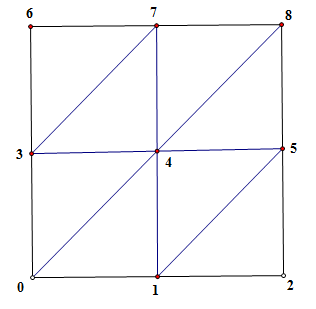
\includegraphics[scale=0.5]{./figures/2.png}
\caption{}
\end{figure}

假设没有经过边界处理的刚度矩阵$A$:
$$
\begin{bmatrix}
a_{00} & a_{01} & a_{02} & a_{03} & a_{04} & a_{05} & a_{06} & a_{07} & a_{08}\\
a_{10} & a_{11} & a_{12} & a_{13} & a_{14} & a_{15} & a_{16} & a_{17} & a_{18}\\
a_{20} & a_{21} & a_{22} & a_{23} & a_{24} & a_{25} & a_{26} & a_{27} & a_{28}\\
a_{30} & a_{31} & a_{32} & a_{33} & a_{34} & a_{35} & a_{36} & a_{37} & a_{38}\\
a_{40} & a_{41} & a_{42} & a_{43} & a_{44} & a_{45} & a_{46} & a_{47} & a_{48}\\
a_{50} & a_{51} & a_{52} & a_{53} & a_{54} & a_{55} & a_{56} & a_{57} & a_{58}\\
a_{60} & a_{61} & a_{62} & a_{63} & a_{64} & a_{65} & a_{66} & a_{67} & a_{68}\\
a_{70} & a_{71} & a_{72} & a_{73} & a_{74} & a_{75} & a_{76} & a_{77} & a_{78}\\
a_{80} & a_{81} & a_{82} & a_{83} & a_{84} & a_{85} & a_{86} & a_{87} & a_{88}\\
\end{bmatrix}
$$

即$$
\begin{bmatrix}
a_{00} & a_{01} & a_{02} & a_{03} & a_{04} & a_{05} & a_{06} & a_{07} & a_{08}\\
a_{10} & a_{11} & a_{12} & a_{13} & a_{14} & a_{15} & a_{16} & a_{17} & a_{18}\\
a_{20} & a_{21} & a_{22} & a_{23} & a_{24} & a_{25} & a_{26} & a_{27} & a_{28}\\
a_{30} & a_{31} & a_{32} & a_{33} & a_{34} & a_{35} & a_{36} & a_{37} & a_{38}\\
a_{40} & a_{41} & a_{42} & a_{43} & a_{44} & a_{45} & a_{46} & a_{47} & a_{48}\\
a_{50} & a_{51} & a_{52} & a_{53} & a_{54} & a_{55} & a_{56} & a_{57} & a_{58}\\
a_{60} & a_{61} & a_{62} & a_{63} & a_{64} & a_{65} & a_{66} & a_{67} & a_{68}\\
a_{70} & a_{71} & a_{72} & a_{73} & a_{74} & a_{75} & a_{76} & a_{77} & a_{78}\\
a_{80} & a_{81} & a_{82} & a_{83} & a_{84} & a_{85} & a_{86} & a_{87} & a_{88}\\
\end{bmatrix}
\begin{bmatrix}
u_{0} \\
u_{1} \\
u_{2} \\
u_{3} \\
u_{4} \\
u_{5} \\
u_{6} \\
u_{7} \\
u_{8} \\
\end{bmatrix}=
\begin{bmatrix}
b_{0} \\
b_{1} \\
b_{2} \\
b_{3} \\
b_{4} \\
b_{5} \\
b_{6} \\
b_{7} \\
b_{8} \\
\end{bmatrix}$$

其中,$B=\begin{bmatrix}
b_{0} \\
b_{1} \\
b_{2} \\
b_{3} \\
b_{4} \\
b_{5} \\
b_{6} \\
b_{7} \\
b_{8} \\
\end{bmatrix}$是没有经过边界处理的载荷向量,$u_0,u_1,u_2,u_3,u_5,u_6,u_7,u_8$是$u$在边界上的已知值。因此有

$$
\begin{cases}
a_{00}u_0 + a_{01}u_1 + a_{02}u_2 + a_{03}u_3 + a_{04}u_{4} + a_{05}u_5 + a_{06}u_6 + a_{07}u_7 + a_{08}u_8=b_0 \\
a_{10}u_0 + a_{11}u_1 + a_{12}u_2 + a_{13}u_3 + a_{14}u_{4} + a_{15}u_5 + a_{16}u_6 + a_{17}u_7 + a_{18}u_8=b_1 \\
a_{20}u_0 + a_{21}u_1 + a_{22}u_2 + a_{23}u_3 + a_{24}u_{4} + a_{25}u_5 + a_{26}u_6 + a_{27}u_7 + a_{28}u_8=b_2 \\
a_{30}u_0 + a_{31}u_1 + a_{32}u_2 + a_{33}u_3 + a_{34}u_{4} + a_{35}u_5 + a_{36}u_6 + a_{37}u_7 + a_{38}u_8=b_3 \\
a_{40}u_0 + a_{41}u_1 + a_{42}u_2 + a_{43}u_3 + a_{44}u_{4} + a_{45}u_5 + a_{46}u_6 + a_{47}u_7 + a_{48}u_8=b_4 \\
a_{50}u_0 + a_{51}u_1 + a_{52}u_2 + a_{53}u_3 + a_{54}u_{4} + a_{55}u_5 + a_{56}u_6 + a_{57}u_7 + a_{58}u_8=b_5 \\
a_{60}u_0 + a_{61}u_1 + a_{62}u_2 + a_{63}u_3 + a_{64}u_{4} + a_{65}u_5 + a_{66}u_6 + a_{67}u_7 + a_{68}u_8=b_6 \\
a_{70}u_0 + a_{71}u_1 + a_{72}u_2 + a_{73}u_3 + a_{74}u_{4} + a_{75}u_5 + a_{76}u_6 + a_{77}u_7 + a_{78}u_8=b_7 \\
a_{80}u_0 + a_{81}u_1 + a_{82}u_2 + a_{83}u_3 + a_{84}u_{4} + a_{85}u_5 + a_{86}u_6 + a_{87}u_7 + a_{88}u_8=8_0 \\
\end{cases}
$$

现在开始对 $A$ 进行边界处理,和一维边界处理一样,首先找到边界点所在的位置,然后把 $A$ 相应的元素变成对角线上为1,对角线元素其他的行和列变成0,其余元素不变。这里$0,1,2,3,5,6,7,8$是边界点,因此

$$
A=\begin{bmatrix}
1 & 0 & 0 & 0 & 0 & 0 & 0 & 0 & 0 \\
0 & 1 & 0 & 0 & 0 & 0 & 0 & 0 & 0 \\
0 & 0 & 1 & 0 & 0 & 0 & 0 & 0 & 0 \\
0 & 0 & 0 & 1 & 0 & 0 & 0 & 0 & 0 \\
0 & 0 & 0 & 0 & a_{44} & 0 & 0 & 0 & 0\\
0 & 0 & 0 & 0 & 0 & 1 & 0 & 0 & 0\\
0 & 0 & 0 & 0 & 0 & 0 & 1 & 0 & 0 \\
0 & 0 & 0 & 0 & 0 & 0 & 0 & 1 & 0 \\
0 & 0 & 0 & 0 & 0 & 0 & 0 & 0 & 1 \\
\end{bmatrix}
$$

$A$ 发生了改变,因此 $B$ 也应当发生改变。

把上面的公式重写成下面的形式

$$
\begin{cases}
u_0 + 0 + 0 + 0 + 0 + 0 + 0 + 0 + 0 = u_0 \\
0 + u_1 + 0 + 0 + 0 + 0 + 0 + 0 + 0 = u_1 \\
0 +  0 + u_2 +0 + 0 + 0 + 0 + 0 + 0 = u_2 \\
0 +  0 + 0 + u_3 +0 + 0 + 0 + 0 + 0 = u_3 \\
a_{44}u_{4} = b_4 -a_{40}u_0 - a_{41}u_1- a_{42}u_2-a_{43}u_3 -a_{45}u_5- a_{46}u_6- a_{47}u_7- a_{48}u_8 \\
0 +  0 + 0 + 0 + u_5 +0 + 0 + 0 + 0 = u_5 \\
0 +  0 + 0 + 0 + 0 +u_6 +0 + 0 + 0 = u_6 \\
0 +  0 + 0 + 0 + 0 + 0 + u_7 +0 + 0 = u_7 \\
0 +  0 + 0 + 0 + 0 + 0 + 0 + u_8 + 0 = u_8 \\
\end{cases}
$$

即
$$
\begin{bmatrix}
1 & 0 & 0 & 0 & 0 & 0 & 0 & 0 & 0 \\
0 & 1 & 0 & 0 & 0 & 0 & 0 & 0 & 0 \\
0 & 0 & 1 & 0 & 0 & 0 & 0 & 0 & 0 \\
0 & 0 & 0 & 1 & 0 & 0 & 0 & 0 & 0 \\
0 & 0 & 0 & 0 & a_{44} & 0 & 0 & 0 & 0\\
0 & 0 & 0 & 0 & 0 & 1 & 0 & 0 & 0\\
0 & 0 & 0 & 0 & 0 & 0 & 1 & 0 & 0 \\
0 & 0 & 0 & 0 & 0 & 0 & 0 & 1 & 0 \\
0 & 0 & 0 & 0 & 0 & 0 & 0 & 0 & 1 \\
\end{bmatrix}
\begin{bmatrix}
u_{0} \\
u_{1} \\
u_{2} \\
u_{3} \\
u_{4} \\
u_{5} \\
u_{6} \\
u_{7} \\
u_{8} \\
\end{bmatrix}=\\
\begin{bmatrix}
u_{0} \\
u_{1} \\
u_{2} \\
u_{3} \\
b_4-a_{40}u_0-a_{41}u_1-a_{42}u_2-a_{43}u_3-a_{45}u_5-a_{46}u_6-a_{47}u_7-a_{48}u_8
u_{5} \\
u_{6} \\
u_{7} \\
u_{8} \\
\end{bmatrix}
$$

其中
$$
B=\begin{bmatrix}
u_{0} \\
u_{1} \\
u_{2} \\
u_{3} \\
b_4-a_{40}u_0-a_{41}u_1-a_{42}u_2-a_{43}u_3-a_{45}u_5-a_{46}u_6-a_{47}u_7-a_{48}u_8 \\
u_{5} \\
u_{6} \\
u_{7} \\
u_{8} \\
\end{bmatrix}
$$
是经过边界处理后的载荷向量



































%坎坎坷坷扩


%\cite{tam19912d}
%\bibliography{../ref}
\end{document}
